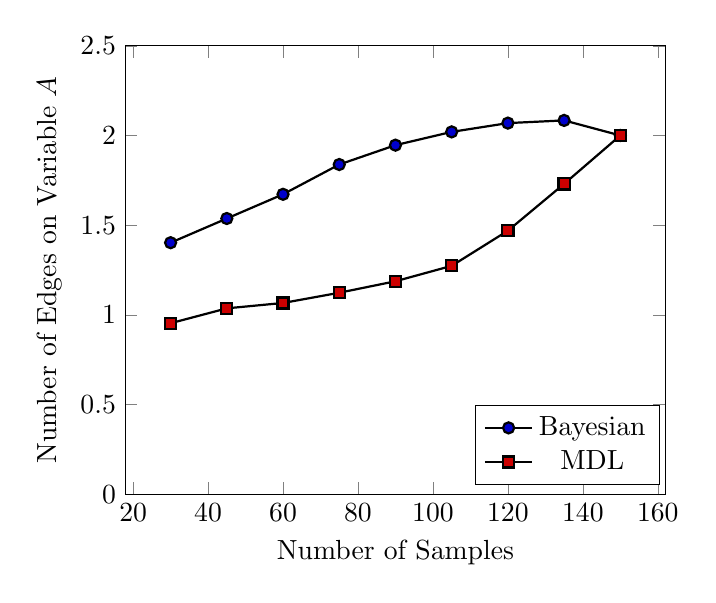
\begin{tikzpicture}
\begin{axis}[
		xlabel = Number of Samples,
		ylabel = Number of Edges on Variable $A$,
		legend style={at={(0.99,0.02)},anchor=south east},
		ymin=0.0, ymax=2.5
]
\addplot+[solid ,black,thick] coordinates {
(30, 1.402)
(45, 1.537)
(60, 1.672)
(75, 1.838)
(90, 1.946)
(105, 2.02)
(120, 2.069)
(135, 2.084)
(150, 2.0)
};
\addlegendentry{Bayesian};

\addplot+[solid ,black,thick] coordinates {
	(30, 0.953)
	(45, 1.036)
	(60, 1.066)
	(75, 1.123)
	(90, 1.187)
	(105, 1.273)
	(120, 1.469)
	(135, 1.730)
	(150, 2.0)
};
\addlegendentry{MDL};
\end{axis}
\end{tikzpicture}
